\documentclass[assignment1.tex]{subfiles}
\begin{document}

\section*{3η Άσκηση}


\subsection{Περιγραφή Προσομοίωσης}
Για την προσομοίωση του πειράματος μέτρησης της επιτάχυνσης της βαρύτητας ακολουθήθηκε η ακόλουθη μέθοδος. Ορίστηκε ένα διάνυσμα $\vec{L}$ με τα μήκη της εκφώνησης. Σε κάθε μήκος $L_i$, γίνεται προσομοίωση μέτρησης της περιόδου. 

Συγκεκριμένα, κάθε μέτρηση περιόδου, θεωρείται πως προκύπτει από την πραγματική περίοδο (\ref{eq:period}), για δοσμένο \textlatin{g} (πχ $9.8\frac{m}{s^2}$) και μήκος $L_i$, στην οποία έχει προστεθεί ένας τυχαίος αριθμός. Δηλαδή η μέτρηση είναι μια τυχαία μεταβλητή $T_i = T + \delta T_i$, όπου $\delta T_i \sim N(0,1)\cdot \delta T$. Τελικά προκύπτει ένα νέο διάνυσμα $\vec{T}$.

\begin{equation}
T = 2\pi \sqrt{\frac{L}{g}}
\label{eq:period}
\end{equation}

Από κάθε ζεύγος τιμών $(L_i, T_i)$ υπολογίζεται έμμεσα η τιμή της επιτάχυνσης της βαρύτητας $g_i$, με σφάλμα που δίνεται από το νόμο διάδοσης σφαλμάτων (\ref{eq:gError}).

\begin{equation}
\delta g_i = 4\pi^2 \sqrt{\left(\frac{\delta L}{T_i^2}\right)^2 + \left(\frac{2L_i\delta T}{T_i^3}\right)^2}, i=1,2,3,4
\label{eq:gError}
\end{equation}

Η μέση τιμή των έμμεσων μετρήσεων της επιτάχυνση της βαρύτητας δίνει μια εκτίμηση για το $g$.

Αν η εξίσωση (\ref{eq:period}) λυθεί ως προς $T^2$, τότε προκύπτει η εξίσωση (\ref{eq:linear}), η οποία είναι μια γραμμική συνάρτηση $T^2(L)$, με τη σταθερά $g$ κρυμμένη μέσα στο συντελεστή διεύθυνσης της ευθείας. 

\begin{equation}
T^2 = \frac{4\pi^2}{g}L
\label{eq:linear}
\end{equation}

Τα ζεύγη $(L_i, T_i)$ μπορούν να χρησιμοποιηθούν για να χαραχτεί μια ευθεία ελαχίστων τετραγώνων, η οποία θα είναι κοντά στην εξίσωση (\ref{eq:linear}). Από την κλίση της ευθείας ελαχίστων τετραγώνων υπολογίζεται το $g$.

To πείραμα προσομοιώνεται δύο φορές, με τη διαφορά ότι στη δεύτερη, υπάρχει ένα σταθερό συστηματικό σφάλμα στη μέτρηση του μήκους του εκκρεμούς, $\delta L_{sys}=0.05m$. Επομένως, αναμένεται η ευθεία ελαχίστων τετραγώνων να είναι μετατοπισμένη κατά $0.05m$ δεξιά.


\subsection{Αποτελέσματα Προσομοίωσης}
Στην προσομοίωση χωρίς συστηματικό σφάλμα, παρήχθησαν τα αποτελέσματα του Πίνακα \ref{table:meas1}. Η μέση τιμή των μετρήσεων της επιτάχυνσης της βαρύτητας δίνει $g=10.5\frac{m}{s^2}$ που είναι πολύ υψηλό. Ωστόσο, η στήλη των σφαλμάτων $\delta g$ δείχνει ότι τα σφάλματα των μετρήσεων ήταν αρκετά μεγάλα, και επομένως δικαιολογούν το αποτέλεσμα.

\begin{table}[ht]
\centering
\begin{tabular}{||c c c ||} 
 \hline
 $L[m]$ & $g[\frac{m}{s^2}]$ & $\delta g$ \\ [0.5ex] 
 \hline\hline
 0.2 & 12 & 3 \\ 
 0.4 & 8 & 1 \\
 0.8 & 11 & 1 \\
 1.0 & 12 & 0 \\ [1ex] 
 \hline
\end{tabular}
\caption{Μετρήσεις χωρίς συστηματικό σφάλμα}
\label{table:meas1}
\end{table}

Με τη μέθοδο ελαχίστων τετραγώνων, προκύπτει $g=12.0\frac{m}{s^2}$, που είναι εξίσου μεγάλο. Η ευθεία ελαχίστων τετραγώνων φαίνεται στο Σχήμα \ref{fig:least_squares}.

Στην προσομοίωση με συστηματικό σφάλμα, παρήχθησαν τα αποτελέσματα του Πίνακα \ref{table:meas2}. Η μέση τιμή των μετρήσεων της επιτάχυνσης της βαρύτητας δίνει $g=9.78\frac{m}{s^2}$ πιο χαμηλό από το πρώτο πείραμα αλλά η στήλη των σφαλμάτων $\delta g$ δείχνει σφάλματα ίδιας τάξης μεγέθους με την πρώτη προσομοίωση.

\begin{table}[ht]
\centering
\begin{tabular}{||c c c ||} 
 \hline
 $L[m]$ & $g[\frac{m}{s^2}]$ & $\delta g$ \\ [0.5ex] 
 \hline\hline
 0.2 & 10 & 2 \\ 
 0.4 & 8 & 1 \\
 0.8 & 10 & 1 \\
 1.0 & 11 & 1 \\ [1ex] 
 \hline
\end{tabular}
\caption{Μετρήσεις με συστηματικό σφάλμα}
\label{table:meas2}
\end{table}


Τέλος, η ευθεία ελαχίστων τετραγώνων δίνει $g=11.6\frac{m}{s^2}$. Η ευθεία ελαχίστων τετραγώνων φαίνεται στο Σχήμα \ref{fig:least_squares}.

Παρατηρείται ότι και στις δύο μεθόδους τα σφάλματα μέτρησης της σταθεράς ήταν πολύ μεγάλα για να εξαχθούν κάποια ασφαλή συμπεράσματα για την τιμή της. Ωστόσο, όπως φαίνεται, η μέθοδος των ελαχίστων τετραγώνων επιδρά θετικά στον περιορισμό της διάδοσης του συστηματικού σφάλματος.

\begin{figure}[hp]
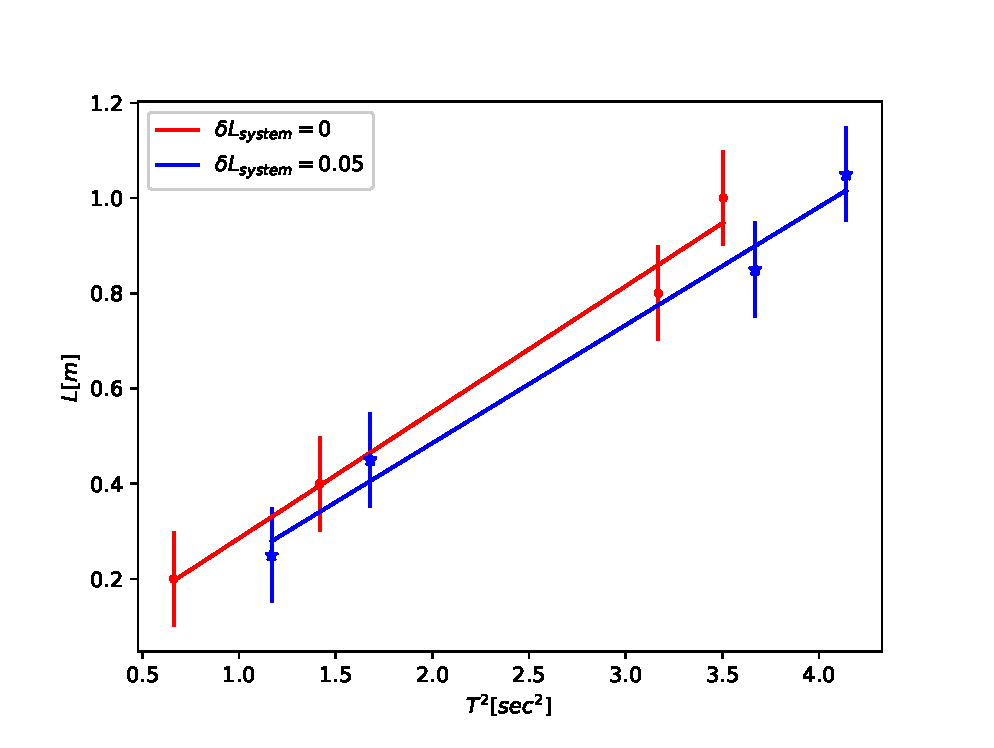
\includegraphics[width=0.9\textwidth]{experiment.eps}
\centering
\caption{Ελάχιστα Τετράγωνα Προσομοίωσης}
\label{fig:least_squares}
\end{figure} 

\FloatBarrier

\subsection{Πηγαίος Κώδικας}

Παρακάτω ακολουθεί ο κώδικας που γράφτηκε σε \textlatin{Python} και έγινε χρήση της βιβλιοθήκης \textlatin{Numpy}.

\selectlanguage{english}
\lstinputlisting[style=python, firstline=8]{mc_experiment.py}

\end{document}